%\documentclass[a4paper,11pt,twoside]{article}
\documentclass[preprint,10pt,numbers]{sigplanconf}
\usepackage[utf8]{inputenc}          % UTF-8 Encoding
\usepackage{hyperref}                % Interactive PDF
\usepackage{float}                   % Float control
\usepackage{multirow}                % Span multiple rows & columns in a table
\usepackage{amsmath}                 % Mathematics library
\usepackage{amssymb}                 % Provides math fonts
\usepackage{amsthm}                  % Provides \newtheorem, \theoremstyle, etc.
\usepackage[T1]{fontenc}             % Fixes font issues
\usepackage{lmodern}
\usepackage{tikz}                    % Drawing
\usetikzlibrary{trees}
\usetikzlibrary{calc}
\usepackage{xcolor}
\usepackage{listings}

\lstset{
 backgroundcolor=\color{white},   % choose the background color; you must add \usepackage{color} or \usepackage{xcolor}
 basicstyle=\ttfamily\small,        % the size of the fonts that are used for the code
 commentstyle=\itshape,
 breakatwhitespace=false,         % sets if automatic breaks should only happen at whitespace
 breaklines=true,                 % sets automatic line breaking
 captionpos=b,                    % sets the caption-position to bottom
 deletekeywords={...},            % if you want to delete keywords from the given language
 escapeinside={§*}{*§},          % if you want to add LaTeX within your code
 extendedchars=true,              % lets you use non-ASCII characters; for 8-bits encodings only, does not work with UTF-8
 frame=none,	                   % adds a frame around the code
 keepspaces=true,                 % keeps spaces in text, useful for keeping indentation of code (possibly needs columns=flexible)
 numbers=none,                    % where to put the line-numbers; possible values are (none, left, right)
 rulecolor=\color{black},         % if not set, the frame-color may be changed on line-breaks within not-black text (e.g. comments (green here))
 showspaces=false,                % show spaces everywhere adding particular underscores; it overrides 'showstringspaces'
 showstringspaces=false,          % underline spaces within strings only
 showtabs=false,                  % show tabs within strings adding particular underscores
 tabsize=2,	                   % sets default tabsize to 2 spaces
 title=\lstname,                   % show the filename of files included with \lstinputlisting; also try caption instead of title
  belowcaptionskip=-1\baselineskip,
  xleftmargin=\parindent
}
% Links style
\lstdefinestyle{links}{
  basicstyle=\linespread{1.0}\ttfamily\footnotesize,
  language=Caml,
  frame=none,
  literate= {+}{{$+$}}1 {*}{{$*$}}1
            {<=}{{$\leq$}}1 {>=}{{$\geq$}}1 
            {=>}{{$\Rightarrow$}}1
            {->}{{$\to$}}1 {~>}{{$\rightsquigarrow$}}1
}
%\usepackage[
%backend=bibtex,
%style=numeric,
%sorting=nyt
%]{biblatex}                   % Bibliography
%\addbibresource{references.bib}


% Convenient macros
\newcommand{\defas}[0]{\mathrel{\overset{\makebox[0pt]{\mbox{\normalfont\tiny\sffamily def}}}{=}}} % "defined-as-equal"

%% Meta-stuff like authors, title, etc.
%\author{Daniel Hillerström\\\small{CDT in Pervasive Parallelism}\\\small{\href{mailto:daniel.hillerstrom@ed.ac.uk}{daniel.hillerstrom@ed.ac.uk}}}
%\date{\today}
%\title{Proposal: Effective Concurrency in Links} % Just some title; change at a later point.

% The document
\makeatletter
\def\@copyrightspace{\relax}
\makeatother
\begin{document}
\title{Effective Concurrency in Links}
%\subtitle{via handlers}

\authorinfo{Daniel Hillerström}
           {CDT Pervasive Parallelism}
           {\href{mailto:daniel.hillerstrom@ed.ac.uk}{daniel.hillerstrom@ed.ac.uk}}
  \maketitle
  \begin{abstract}
    An abstract will appear here\dots
  \end{abstract}
  \raggedbottom
  % Input the content
  \section{Introduction}
Run-time scheduling is a domain-specific problem as the performance goal of a scheduler can be paramount to the overall performance of a program. Consequently, schedulers employ different metrics to measure performance. For example, \emph{high-throughput} schedulers seek to optimise the throughput of jobs \cite{Berman2003}, hence performance might be measured by the number of jobs processed by the system. Criteria such as fairness or utilisation might be used to measure the performance of \emph{resource} schedulers as they seek to coordinate accesses to shared resources \cite{Berman2003}. Furthermore, \emph{high-performance} schedulers seek to minimise execution time for a single program. In this case performance is measured by the raw execution speed.

Thus scheduling is important. However, scheduling is often the responsibility of the compiler writer, but the concern of the application programmer. For example, grid-based computations may benefit from neighbouring points being scheduled together. Yet the programmer has little or no say about the matter as schedulers typically are baked into the run-time system \cite{Dolan2015}. 

We propose to rectify this mismatch by transferring the responsibility for scheduling to the application programmer. Concretely, we propose to abstract over the choice of scheduling by adapting the approach taken by Multicore OCaml \cite{Dolan2015} to use Plotkin and Pretnar's \emph{handlers for algebraic effects} \cite{Plotkin2013} to encode concurrency primitives. Specifically, we plan implement a backend for the functional programming language Links \cite{Cooper2006}, and take advantage of its existing implementation of algebraic effect handlers \cite{Hillerstrom2015} to encode Links' concurrency primitives.

  % Plotkin and Power's algebraic effects \cite{Plotkin2001} combined with Plotkin and Pretnar's handlers \cite{Plotkin2013} yield a programming model for controlling computational effects. An algebraic effect is a collection of abstract operations without predefined semantics. Handlers interpret algebraic effects by assigning semantics to abstract operations. Thus, the control of computational effects is lifted from the run-time system into the hands of the programmer. Clearly, it shifts additional responsibility onto the programmer, however, in addition it opens up a design space that was previously secluded from the programmer. Now, the programmer may extend the capabilities of the run-time system beyond what the language implementor envisaged.

  % For example, it is well-known that concurrency primitives can be encoded through algebraic effects \cite{Bauer2015,Dolan2015} as spawning a new thread is an effect. Furthermore, suspending a thread is an effect. Handlers of these effects are schedulers. Hence, the programmer is free to implement a particular scheduling policy tailored for the application. The choice of scheduler can have significant impact on performance as a scheduler's performance goal can be paramount to the overall performance of an application \cite{Berman2003}.

  % However\dots

  \section{Problem definition}\label{sec:problemdefinition}
%  Although, handlers for algebraic effects have many practical applications \cite{Kammar2013,Bauer2015,Hillerstrom2015,Dolan2015}, there does not yet exist an efficient implementation of handlers. Multicore OCaml implements linear handlers which only allow the continuation invoked once. This restriction is enforced during run-time. Furthermore, because OCaml lacks an effect system\dots
Run-time scheduling is recognised as an important problem for performance \cite{Augonnet2011,Augonnet2012,Agullo2015}. In particular in the field of high-performance computing where scheduling is concerned about exploiting heterogeneity to accelerate computations. There already exists many tools that attempt to solve this problem, e.g. CellSs \cite{Bellens2009}, StarSS \cite{Planas2009}, StarPU \cite{Augonnet2011}, QUARK \cite{YarKhan2011}, PaRSEC \cite{Bosilca2013} to mention a few.\footnote{These tools are further discussed in Section \ref{sec:tools}.}

These tools take a common approach to scheduling: Given a task-graph-based description of a program, they will attempt to map individual tasks onto computational devices. Most of the tools seek to do this mapping automatically.

However, the key observation is, that, the aforementioned tools provide weak abstractions that makes scheduling non-modular. Support for schedulers is added by resorting to compile-time meta programming in a foreign language such as \texttt{pragmas}. Hence, schedulers become tightly coupled with computations. Consequently, it is nontrivial to reuse a particular scheduler or change scheduler.
% Moreover, the programmer still has a limited say.
% End up with a monolithic tools

Ideally, we would want schedulers to be first-class citizens in the host language. Therefore, we ask the following question:
\begin{center}
  \emph{How may we reify schedulers as an integrated host language construct?}
\end{center}
In Section \ref{sec:proposedsolution} we give propose an answer to the above question.

  \section{Proposed solution}\label{sec:proposedsolution}
The main observation is, that, tools often happen to offer poor abstractions which requires the programmer to annotate or describe code in \emph{a foreign language}. As a consequence code becomes non-modular, and thus, it difficult to combine different pieces of code.

We propose to an approach along the lines of Multicore OCaml to use algebraic effect handlers to encode concurrency directly in the host language. Plotkin and Power's algebraic effects \cite{Plotkin2001} are collections of abstract operations without predefined semantics. Plotkin and Pretnar's handlers \cite{Plotkin2013} assign semantics to abstract operations. Thus this programming model provide a clear separation of effects and their interpretations.

The key observation is that concurrency primitives are encodable as algebraic effects \cite{Bauer2015,Dolan2015}. 

\subsection{Example: Cooperative multitasking}
It is straightforward to encode \emph{cooperative multitasking} using the following two operations:
\begin{itemize}
  \item $\text{fork} : (() \to a) \to F a$
  \item $\text{yield} : ()$
\end{itemize}
The first operation \emph{fork} takes a computation as input, and returns a future which eventually will contain the result of the said computation. The second operation \emph{yield} suspends the computation which it is invoked inside. Using these operations we can easily define an asynchronous computation that computes the $n$th Fibonacci number, e.g. 
\begin{lstlisting}[style={links},caption={}]
fun fib(n) {
  if (n <= 1) {n}
  else {
    var f1 = fork(fun() { fib(n-1) });
    var f2 = fork(fun() { fib(n-2) });
    get(f1) + get(f2)
  }
}
\end{lstlisting}
where \texttt{get} attempts to retrieve the value inside a future. Its implementation is omitted here, but it is simple to implement in terms of yield.\footnote{The full source code is available at \url{https://github.com/dhil/mscr-dissertation/proposal/coroutines.links}} Next, we define a breadth-first scheduler:
\begin{lstlisting}[style={links},caption={}]
open handler bfscheduler(m)(f) {
  case Fork(t,k) -> {
   var new_f = new_future();
   enqueue(fun(_) { scheduler(t)(Just(new_f))() });
   k(new_f)(f)
  }
  case Yield(k)  -> { 
   enqueue(fun(_) { k(())(f) }); 
   var t = dequeue(); t(()) 
  }
  case Return(x) -> {
     put(f,x);
     if (is_empty()) { x }
     else { var t = dequeue(); t(()) }
   } 
}
\end{lstlisting}
The handler \texttt{bfscheduler} implements a scheduler by pattern matching on occurrences of operations \texttt{Fork} and \texttt{Yield} in some computation \texttt{m}. The handler is parameterised by a future \texttt{f}. For instance, when \texttt{fork} occurs in \texttt{fib} the \texttt{bfscheduler} first allocates a new future \texttt{new\_f}. Then it recursively schedules the forked computation \texttt{t} to run later. Finally, it resumes the computation in which \texttt{t} was forked by invokng the continuation \texttt{k} with the new future \texttt{new\_f}, the previous future \texttt{f} is saved for the next invocation of the scheduler. Observe, that on a single-core platform this scheduler effectively defers execution of forked computations.

Upon an occurrence of \texttt{yield} in \texttt{m} the handler suspends the computation and schedules it to run later. Thereafter it dequeues and resumes another computation \texttt{t}.

Finally, when a computation finishes the handler puts the return value inside the future \texttt{f}. Furthermore, if the computation queue is nonempty it dequeues and resumes another computation, otherwise it the return value of latest computation is returned.
\begin{figure}
\begin{center}
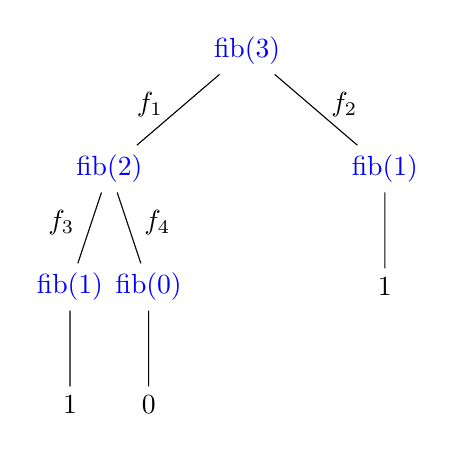
\begin{tikzpicture}[level distance=1.5cm,
level 1/.style={sibling distance=3.5cm},
level 2/.style={sibling distance=1cm}]
%\tikzstyle{every node}=[circle,draw]

\node (Root) [blue,rectangle] {fib(3)}
    child { node[blue] (q0) {fib(2)} 
      child { node[blue] (q00) {fib(1)}
        child { node[draw=none] {1} }
        edge from parent node [draw=none,left,xshift=-2.0,yshift=2.0] {$f_3$}
      }
      child { node[blue] (q01) {fib(0)} 
        child { node[draw=none] {0}         
        }
        edge from parent node [draw=none,right,xshift=2.0,yshift=2.0] {$f_4$}
      }
      edge from parent node [draw=none,left,xshift=-2.0,yshift=2.0] {$f_1$}
    }
    child { node [blue] (q1) {fib(1)}
      child { node[draw=none] (q10) {1}
      }
      edge from parent node [draw=none,right,xshift=2.0,yshift=2.0] {$f_2$}
    };
\end{tikzpicture}\caption{Computation tree of \texttt{fib(3)} when employing breadth-first scheduling.}\label{fig:bfs}
\end{center}
\end{figure}

This scheduler is suboptimal for the Fibonacci-computation on single-core platform, because it materialises it entire computation tree of \texttt{fib}. Figure \ref{fig:bfs} depicts the computation tree for \texttt{fib($3$)}. The labels $f_i$ indicate the order in which tasks are created.

\begin{figure}
\begin{center}
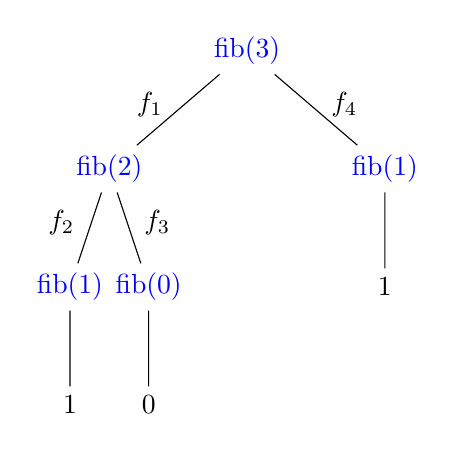
\begin{tikzpicture}[level distance=1.5cm,
level 1/.style={sibling distance=3.5cm},
level 2/.style={sibling distance=1cm}]
%\tikzstyle{every node}=[circle,draw]

\node (Root) [blue,rectangle] {fib(3)}
    child { node[blue] (q0) {fib(2)} 
      child { node[blue] (q00) {fib(1)}
        child { node[draw=none] {1} }
        edge from parent node [draw=none,left,xshift=-2.0,yshift=2.0] {$f_2$}
      }
      child { node[blue] (q01) {fib(0)} 
        child { node[draw=none] {0}         
        }
        edge from parent node [draw=none,right,xshift=2.0,yshift=2.0] {$f_3$}
      }
      edge from parent node [draw=none,left,xshift=-2.0,yshift=2.0] {$f_1$}
    }
    child { node [blue] (q1) {fib(1)}
      child { node[draw=none] (q10) {1}
      }
      edge from parent node [draw=none,right,xshift=2.0,yshift=2.0] {$f_4$}
    };
\end{tikzpicture}\caption{Computation tree of \texttt{fib(3)} when employing depth-first scheduling.}\label{fig:dfs}
\end{center}
\end{figure}
  \section{Background}\label{sec:background}
  \subsection{Scheduling tools}\label{sec:tools}
There exists numerous tools that attempt to address the problem of scheduling in high-performance computing; a selection of these tools were briefly outlined in Section \ref{sec:problemdefinition}.
  \subsection{Links programming language}
  Links is a strongly, statically typed functional programming language oriented towards web-programming \cite{Cooper2006}. Notably, Links implements effect handlers as first-class citizens \cite{Hillerstrom2015}. Moreover, the implementation support both deep and shallow handlers. However, since Links is an interpreted language the performance of handlers is low.

  \subsection{Optimisation of single-shot continuations}

  \subsection{Handlers implementations}
  This section briefly surveys existing implementations of effect handlers. Section \ref{sec:first-class} considers languages with first-class handlers, whilst Section \ref{sec:library} discusses embeddings of handlers in the pure functional programming language Haskell.
  \subsubsection{First-class implementations}\label{sec:first-class}
  \begin{table}[H]
    \centering 
    \begin{tabular}{| l | l | l |}
      \hline
      \multicolumn{1}{|c|}{Language} & \multicolumn{1}{c|}{Handlers} & \multicolumn{1}{c|}{Developed by} \\
      \hline
      Eff & Deep handlers & Bauer and Pretnar \\ 
      \hline
      Frank & Shallow handlers & McLaughlin, Lindley and McBride \\    
      \hline
      Links & Shallow and deep handlers & Hillerström and Lindley\\
      \hline
      Multicore OCaml & Deep handlers & OCamlLabs \\
      \hline    
    \end{tabular}\caption{Languages with first-class effect handlers.}\label{tbl:impls}
  \end{table}
  Table \ref{tbl:impls} provide an overview of languages where effect handlers are first-class citizens. 

The Eff language is a OCaml-style language with deep handlers. It support for effect polymorphism through subtyping \cite{Bauer2015}. 
The functional programming Links implements both deep and shallow handlers \cite{Hillerstrom2015}. Moreover, the implementation supports effect polymorphism through Links' existing row polymorphic effect system.
    
  \subsubsection{Library implementations}\label{sec:library}

  \section{Evaluation}
  The primary metric for evaluation of the proposed solution will be performance. As discussed earlier there are various metrics for measuring performance. We intend to mainly measure performance by raw execution speed. Furthermore, we intend to compare our performance results against results for similar programs written in C since it is considered a ``performant'' language. 

Additionally, we will consider the safety of our solution, i.e. which static guarantees, if any, can we exhibit. In order to evaluate safety we intend to give a formal proof of the said properties.

Furthermore, we would like to qualitatively assess the ease of use, that is, whether the handler abstraction makes concurrent programming easier.

  \section{Project feasibility}
  \subsection{Risk analysis}

  \subsection{Project plan}
  \begin{table}[H]
    \centering
    \begin{tabular}{ | l | c | c | c | c | c | }
      \hline
      \multicolumn{1}{|c|}{Activity / Weeks} & 2-4 & 5-9 & 10-17 & 18-21 & 22-33 \\
      \hline
      Prototyping    & X & X & & & \\
      \hline
      Implementation & X & X & X & X & X \\
      \hline
      Testing        & X & X & X & X & X \\
      \hline
      Evaluation     &   &   & X & X & X \\
      \hline
      Related work   &   & X & X &   & X \\
      \hline
      Exam period    &   &   &   & X &   \\
      \hline
      Write up       & X & X & X & X & X  \\
      \hline
    \end{tabular}\caption{Activity overview.}
  \end{table}
  % Bibliography
\bibliographystyle{abbrvnat}
\softraggedright
\nocite{*}
\bibliography{references}
%  \printbibliography[heading=bibintoc]
\end{document}